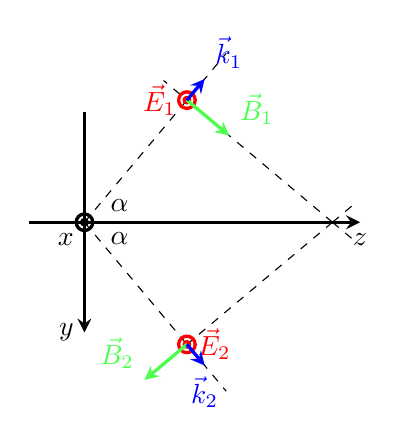
\begin{tikzpicture}[line width = 1.2pt, line join=round,>=stealth,scale=.7]
	\draw [->] (-1,0,0) -- (5,0,0) node[anchor=north] {$z$};
	\draw [->] (0,2,0) -- (0,-2,0) node[anchor=east] {$y$};
	\draw (0,0) circle (1.5 mm);
	\draw (0,0) circle (.5 mm) node[anchor=north east]{$x$};

	\draw[thin,dashed] (0,0) -- (50:4);
	\draw[thin,dashed] (0,0) -- (-50:4);

	\draw[thin,dashed] (4.5,0) -- +(140:4);
	\draw[thin,dashed] (4.5,0) -- +(-140:4);
	\draw[thin,dashed] (4.5,0) -- +(-40:.5);
	\draw[thin,dashed] (4.5,0) -- +(40:.5);

	\centerarc[thin,dotted](0,0)(0:50:1);
	\node at (25:0.7) {$\alpha$};
	\centerarc[thin,dotted](0,0)(0:-50:1);
	\node at (-25:0.7) {$\alpha$};

	\draw[red] (1.859,2.216) circle (1.5 mm);
	\draw[red] (1.859,2.216) circle (.5 mm) node[anchor=east]{$\vec{E}_1$};
	\draw[green!70, ->] (1.859,2.216) -- +(-40:1) node[anchor=south west]{$\vec{B}_1$};
	\draw[blue, ->] (1.859,2.216) -- +(50:.5) node[anchor=south west]{$\vec{k}_1$};

	\draw[red] (1.859,-2.216) circle (1.5 mm);
	\draw[red] (1.859,-2.216) circle (.5 mm) node[anchor=west]{$\vec{E}_2$};
	\draw[green!70, ->] (1.859,-2.216) -- +(-140:1) node[anchor=south east]{$\vec{B}_2$};
	\draw[blue, ->] (1.859,-2.216) -- +(-50:.5) node[anchor=north]{$\vec{k}_2$};

\end{tikzpicture}